\documentclass[10pt]{article}
\usepackage[utf8]{inputenc}
\usepackage[T1]{fontenc}
\usepackage{graphicx}
\usepackage[export]{adjustbox}
\graphicspath{ {./images/} }
\usepackage{amsmath}
\usepackage{amsfonts}
\usepackage{amssymb}
\usepackage[version=4]{mhchem}
\usepackage{stmaryrd}
\usepackage{hyperref}
\hypersetup{colorlinks=true, linkcolor=blue, filecolor=magenta, urlcolor=cyan,}
\urlstyle{same}
\usepackage{kotex}
\usepackage[margin=1in]{geometry}
\parskip=3ex

\title{
 $15213,20xx$년 가을 \\
 어택랩 : 버퍼 오버플로 버그 이해하기 \\
 출시일: x월 x일, 마감일: x월 x일(수) 오후 xx시 xx분}

\author{}
\date{}


\begin{document}
\maketitle
\section*{1 소개}
이 과제에서는 서로 다른 보안 취약점을 가진 두 프로그램에 대해 총 5개의 공격을 생성해야 합니다. 이 실습을 통해 얻을 수 있는 결과는 다음과 같습니다:

\begin{itemize}
  \item 프로그램이 버퍼 오버플로로부터 충분히 보호되지 않을 때 공격자가 보안 취약점을 악용할 수 있는 다양한 방법을 배웁니다.
\item 이를 통해 더 안전한 프로그램을 작성하는 방법과 컴파일러 및 운영체제에서 프로그램을 덜 취약하게 만들기 위해 제공하는 몇 가지 기능을 더 잘 이해할 수 있습니다.
\item x86-64 머신 코드의 스택 및 매개변수 전달 메커니즘에 대해 더 깊이 이해할 수 있습니다.
\item x86-64 명령어가 인코딩되는 방식을 더 깊이 이해할 수 있습니다.
 \item gdb 및 objdump와 같은 디버깅 도구에 대해 더 많은 경험을 쌓을 수 있습니다.
\end{itemize}

\noindent
참고: 이 실습에서는 운영 체제 및 네트워크 서버의 보안 취약점을 악용하는 데 사용되는 방법을 직접 경험하게 됩니다. 이 실습의 목적은 프로그램의 런타임 작동에 대해 배우고 이러한 보안 취약점의 특성을 이해하여 시스템 코드를 작성할 때 이를 방지할 수 있도록 돕는 것입니다. 우리는 시스템 리소스에 대한 무단 액세스를 얻기 위해 다른 형태의 공격을 사용하는 것을 용납하지 않습니다.

\noindent
이 실습을 위한 참고 자료로 CS:APP3e 책의 3.10.3 및 3.10.4 절을 공부하는 것이 좋습니다.

\section*{2 구성}
평소와 마찬가지로 이것은 개별 프로젝트입니다. 여러분을 대상으로 생성된 프로그램에 대한 공격을 생성하게 됩니다.

\subsection*{2.1 파일 가져오기}
여러분의 파일은 브라우저를 다음 주소로 가리키는 것으로 얻을 수 있습니다:

\begin{verbatim}
http://$Attacklab::SERVER_NAME:15513/

INSTRUCTOR: $Attacklab::SERVER_NAME is the machine that runs the
attacklab servers. You define it in attacklab/Attacklab.pm and in
attacklab/src/build/driverhdrs.h
\end{verbatim}

\noindent
서버가 파일을 빌드하여 타겟 k.tar라는 타겟 파일로 브라우저에 반환합니다(여기서 k는 타겟 프로그램의 고유 번호입니다).

\noindent
참고: 타겟을 빌드하고 다운로드하는 데 몇 초 정도 걸리므로 조금만 기다려주세요.

\noindent
작업할 (보호된) Linux 디렉터리에 대상 k.tar 파일을 저장합니다. 그런 다음 다음과 같은 명령을 실행합니다: tar -xvf target k.tar. 아래에 설명된 파일이 포함된 디렉터리 target k가 추출됩니다.

\noindent
한 세트의 파일만 다운로드해야 합니다. 어떤 이유로 여러 개의 대상을 다운로드하는 경우 작업할 대상 하나를 선택하고 나머지는 삭제하세요.

\noindent
경고: Winzip과 같은 유틸리티를 사용하거나 브라우저에서 추출을 수행하도록 허용하여 PC에서 대상 k.tar를 확장하면 실행 파일의 권한 비트가 재설정될 위험이 있습니다.

\noindent
타겟 k의 파일에는 다음이 포함됩니다:
\noindent
README.txt: 디렉터리의 내용을 설명하는 파일입니다.
\noindent
ctarget: 코드 인젝션 공격에 취약한 실행 프로그램입니다.
\noindent
rtarget: 리턴 지향 프로그래밍 공격에 취약한 실행 프로그램입니다.
\noindent
cookie.txt: 공격에서 고유 식별자로 사용할 8자리 16진수 코드입니다.
\noindent
farm.c: 리턴 지향 프로그래밍 공격을 생성하는 데 사용할 공격 대상의 '가젯 팜'의 소스 코드입니다.
\noindent
hex2raw: 공격 문자열을 생성하는 유틸리티입니다. 
\noindent
다음 지침에서는 보호된 로컬 디렉터리에 파일을 복사하고 해당 로컬 디렉터리에서 프로그램을 실행하는 것으로 가정합니다.

\subsection*{2.2 중요 포인트}
다음은 이 실습에 유효한 솔루션에 관한 몇 가지 중요한 규칙을 요약한 것입니다. 이 문서를 처음 읽을 때는 이러한 사항이 크게 이해되지 않을 수 있습니다. 일단 시작하면 규칙의 중심 참조 자료로 여기에 제시되어 있습니다.

\begin{itemize}
\item 타겟을 생성한 컴퓨터와 유사한 컴퓨터에서 과제를 수행해야 합니다.
  \item 여러분의 솔루션은 프로그램의 유효성 검사 코드를 우회하기 위해 공격을 사용해서는 안 됩니다. 특히, ret 명령어에서 사용하기 위해 공격 문자열에 통합하는 모든 주소는 다음 대상 중 하나에 대한 주소여야 합니다:
  \item touch1, touch2 또는 touch3 함수의 주소.
  \item 삽입된 코드의 주소
  \item 가젯 팜에 있는 가젯 중 하나의 주소
  \item start\_farm과 end\_farm 함수에 대한 주소 사이의 주소로만 rtarget 파일에서 가젯을 구성할 수 있습니다.
\end{itemize}

\section*{3 타겟 프로그램}
CTARGET과 RTARGET은 모두 표준 입력에서 문자열을 읽습니다. 아래에 정의된 getbuf 함수를 사용하여 이를 수행합니다:

\begin{verbatim}
unsigned getbuf()
{  
    char buf[BUFFER_SIZE];
    Gets(buf);
    return 1;
}
\end{verbatim}
\noindent
Gets 함수는 표준 라이브러리 함수 gets와 유사하며, 표준 입력('\\n' 또는 파일 끝으로 종료)에서 문자열을 읽고 지정된 대상에 널 종결자와 함께 저장합니다. 이 코드에서 대상은 BUFFER\_SIZE 바이트가 있는 것으로 선언된 배열 buf임을 알 수 있습니다. 타깃이 생성될 당시 BUFFER\_SIZE는 프로그램 버전에 따라 달라지는 컴파일 타임 상수였습니다.
\noindent
함수 Gets() 및 gets()는 대상 버퍼가 읽은 문자열을 저장할 수 있을 만큼 충분히 큰지 확인할 방법이 없습니다. 단순히 바이트 시퀀스를 복사하기 때문에 대상에 할당된 공간의 한계를 초과할 수 있습니다.
\noindent
사용자가 입력하고 getbuf가 읽은 문자열이 충분히 짧으면 다음 실행 예제에서 볼 수 있듯이 getbuf가 1을 반환할 것이 분명합니다:

\begin{verbatim}
    unix> . /ctarget
    Cookie: 0x1a7dd803
    Type string: Keep it short!
    No exploit. Getbuf returned 0x1
    Normal return
\end{verbatim}
\noindent
대체로 긴 문자열을 입력하면 에러가 발생합니다:

\begin{verbatim}
    unix> ./ctarget
    Cookie: 0x1a7dd803
    Type string: This is not a very interesting string, but it has the property ...
    Ouch!: You caused a segmentation fault!
    Better luck next time
\end{verbatim}
\noindent
(표시된 쿠키의 값은 사용자의 쿠키 값과 다를 수 있습니다.) RTARGET 프로그램도 동일한 동작을 합니다. 오류 메시지에서 알 수 있듯이 버퍼를 오버런하면 일반적으로 프로그램 상태가 손상되어 메모리 액세스 오류가 발생합니다. 여러분의 임무는 CTARGET과 RTARGET에 제공하는 문자열을 더 영리하게 사용하여 더 흥미로운 작업을 수행하도록 하는 것입니다. 이를 익스플로잇 문자열이라고 합니다.
\noindent
CTARGET과 RTARGET은 모두 여러 가지 명령줄 인수를 받습니다:
\noindent
-h : 사용 가능한 명령줄 인수 목록 출력
\noindent
-q : 결과를 채점 서버로 전송하지 않음
\noindent
-i FILE: 표준 입력이 아닌 입력된 파일에서 입력값 제공
\noindent
익스플로잇 문자열에는 일반적으로 문자를 인쇄하기 위한 ASCII 값과 일치하지 않는 바이트 값이 포함됩니다. HEX2RAW 프로그램을 사용하면 이러한 원시 문자열을 생성할 수 있습니다. HEX2RAW 사용 방법에 대한 자세한 내용은 부록 A를 참조하세요.

\section*{중요 포인트:}
\begin{itemize}
 \item 익스플로잇 문자열의 중간 위치에 바이트 값 0x0a가 포함되어서는 안 되는데, 이는 개행('\\n')의 ASCII 코드이기 때문입니다. Gets에서 이 바이트가 발견되면 사용자가 문자열을 종료하려고 한 것으로 간주합니다.
  \item HEX2RAW는 하나 이상의 공백으로 구분된 두 자리 16진수 값을 기대합니다. 따라서 16진수 값이 0인 바이트를 생성하려면 00으로 작성해야 합니다. 0xdeadbeef라는 단어를 만들려면 "ef be ad de"를 HEX2RAW에 전달해야 합니다(리틀 엔디안 바이트 순서에 필요한 반전에 유의하세요).
\end{itemize}
\noindent
레벨 중 하나를 올바르게 풀면 다음처럼 대상 프로그램에서 자동으로 채점 서버로 알림을 보냅니다:

\begin{verbatim}
    unix> ./hex2raw < ctarget.l2.txt | ./ctarget
    Cookie: 0x1a7dd803
    Type string:Touch2!: You called touch2(0x1a7dd803)
    Valid solution for level 2 with target ctarget
    PASSED: Sent exploit string to server to be validated.
    NICE JOB!
\end{verbatim}

\begin{center}
\begin{tabular}{|c|l|c|c|c|c|}
\hline
Phase & Program & Level & Method & Function & Points \\
\hline
1 & CTARGET & 1 & CI & touch1 & 10 \\
2 & CTARGET & 2 & CI & touch2 & 25 \\
3 & CTARGET & 3 & CI & touch3 & 25 \\
\hline
4 & RTARGET & 2 & ROP & touch2 & 35 \\
5 & RTARGET & 3 & ROP & touch3 & 5 \\
\hline
\end{tabular}

CI: Code injection

ROP: Return-oriented programming
\end{center}

Figure 1: 어택랩 페이즈의 요약
\noindent
서버는 익스플로잇 문자열을 테스트하여 실제로 작동하는지 확인하고, 사용자 ID(익명성을 위해 타겟 번호로 나열됨)가 이 단계를 완료했음을 나타내는 Attacklab 스코어보드 페이지를 업데이트합니다.
\noindent
브라우저를 다음 주소로 가리키면 스코어보드를 볼 수 있습니다.

\begin{verbatim}
    http://$Attacklab::SERVER_NAME:15513/scoreboard
\end{verbatim}
\noindent
폭탄랩과 달리 이 실습에서는 실수를 해도 불이익이 없습니다. 원하는 문자열로 자유롭게 CTARGET과 RTARGET을 실행해 보세요.
\noindent
중요 참고: 모든 Linux 컴퓨터에서 솔루션을 작업할 수 있지만, 솔루션을 제출하려면 다음 컴퓨터 중 하나에서 실행 중이어야 합니다:

\begin{verbatim}
    INSTRUCTOR: Insert the list of the legal domain names that you established in buflab/src/config.c.
\end{verbatim}
\noindent
그림 1은 실험실의 다섯 단계를 요약한 것입니다. 그림에서 볼 수 있듯이 처음 세 단계는 CTARGET에 대한 코드 인젝션(CI) 공격이고, 마지막 두 단계는 RTARGET에 대한 리턴 지향 프로그래밍(ROP) 공격입니다.

\section*{4 Part I: 코드 인젝션 공격}
처음 세 단계 동안 익스플로잇 스트링은 CTARGET을 공격합니다. 이 프로그램은 실행할 때마다 스택 위치가 일관되게 유지되고 스택의 데이터가 실행 코드로 취급될 수 있도록 설정되어 있습니다. 이러한 특징 때문에 익스플로잇 문자열에 실행 코드의 바이트 인코딩이 포함된 공격에 취약합니다.

\subsection*{4.1 Level 1}
1단계에서는 새로운 코드를 삽입하지 않습니다. 대신 익스플로잇 문자열이 기존 프로시저를 실행하도록 프로그램을 리디렉션합니다.
\noindent
함수 getbuf는 다음 C 코드가 포함된 함수 테스트에 의해 CTARGET 내에서 호출됩니다:

\begin{verbatim}
void test()
{
    int val;
    val = getbuf();
    printf("No exploit. Getbuf returned 0x%x\n", val);
}
\end{verbatim}
\noindent
getbuf가 return문(getbuf의 5행)을 실행하면 프로그램은 일반적으로 함수 테스트(이 함수의 5행) 내에서 실행을 재개합니다. 우리는 동작을 변경하고 싶습니다. ctarget 파일 내에 다음과 같은 C 표현을 가진 touch1 함수에 대한 코드가 있습니다:

\begin{verbatim}
void touch1()
{
    vlevel = 1; /* Part of validation protocol */
    printf("Touch1!: You called touch1()\n");
    validate(1);
    exit(0);
}
\end{verbatim}
\noindent
여러분의 임무는 getbuf가 반환 문을 실행할 때 테스트에 복귀하지 않고 터치 1에 대한 코드를 실행하도록 CTARGET을 가져오는 것입니다. 익스플로잇 문자열이 이 단계와 직접 관련이 없는 스택의 일부도 손상시킬 수 있지만, touch 1은 프로그램이 바로 종료되므로 문제가 되지 않습니다.
\noindent
조언:

\begin{itemize}
\item 이 레벨에 대한 익스플로잇 문자열을 고안하는데 필요한 모든 정보는 CTARGET의 디스어셈블된 버전을 검사하여 확인할 수 있습니다. 이 디스어셈블된 버전을 얻으려면 objdump - d를 사용합니다.
  \item 이 아이디어는 touch 1의 시작 주소의 바이트 표현을 배치하여 getbuf 코드 끝에 있는 ret 명령이 touch 1로 제어권을 이전하도록 하는 것입니다.
  \item 바이트 순서에 주의하세요.
  \item 프로그램이 올바르게 실행되고 있는지 확인하기 위해 GDB를 사용하여 getbuf의 마지막 몇 개의 명령어를 단계별로 실행할 수 있습니다.
  \item getbuf의 스택 프레임 내에서 buf의 배치는 컴파일 시간 상수 BUFFER\_SIZE의 값과 GCC에서 사용하는 할당 전략에 따라 달라집니다. 위치를 확인하려면 디스어셈블된 코드를 살펴봐야 합니다.
\end{itemize}

\subsection*{4.2 Level 2}
2단계는 익스플로잇 문자열의 일부로 소량의 코드를 삽입하는 단계입니다.
\noindent
ctarget 파일 안에는 다음과 같은 C로 표현되는 touch2 함수에 대한 코드가 있습니다:

\begin{verbatim}
void touch2(unsigned val)
{
    vlevel = 2; /* Part of validation protocol */
    if (val == cookie) {
        printf("Touch2!: You called touch2(0x%.8x)\n", val);
        validate(2);
    } else {
        printf("Misfire: You called touch2(0x%.8x)\n", val);
        fail(2);
    }
    exit(0);
}
\end{verbatim}
\noindent
여러분의 임무는 test로 리턴하지 않고 CTARGET이 touch 2에 대한 코드를 실행하도록 하는 것입니다. 하지만 이 경우에는 쿠키를 인수로 전달한 것처럼 touch 2에 표시되도록 해야 합니다.
\noindent
조언:

\begin{itemize}
\item 삽입된 코드의 주소에 대한 바이트 표현을 배치하여 getbuf에 대한 코드 끝에 있는 ret 명령이 제어권을 이 주소로 전송할 수 있도록 해야 합니다.
  \item 함수의 첫 번째 인수는 레지스터 \%rdi에서 전달된다는 것을 기억하세요.
  \item 삽입된 코드는 레지스터를 쿠키로 설정한 다음 ret 명령을 사용하여 터치2의 첫 번째 명령으로 제어를 전송해야 합니다.
  \item 익스플로잇 코드에서 jmp 또는 call 명령을 사용하지 마세요. 이러한 인스트럭션의 대상 주소 인코딩은 공식화하기 어렵습니다. call에서 돌아오지 않는 경우에도 모든 제어권 전송에는 ret 명령을 사용하세요.
  \item 부록 B에서 도구를 사용하여 명령어 시퀀스의 바이트 수준 표현을 생성하는 방법에 대한 설명을 참조하세요.
\end{itemize}

\subsection*{4.3 Level 3}
3단계 역시 코드 인젝션 공격을 포함하지만 인자로 문자열을 전달합니다.
\noindent
ctarget 파일에는 다음과 같은 C 표현을 가진 hexmatch 및 touch 3 함수에 대한 코드가 있습니다:

\begin{verbatim}
/* Compare string to hex represention of unsigned value */
int hexmatch(unsigned val, char *sval)
{
    char cbuf[110];
    /* Make position of check string unpredictable */
    char *s = cbuf + random() % 100;
    sprintf(s, "%.8x", val);
    return strncmp(sval, s, 9) == 0;
}

void touch3(char *sval)
{
    vlevel = 3; /* Part of validation protocol */
    if (hexmatch(cookie, sval)) {
    printf("Touch3!: You called touch3(\"%s\")\n", sval);
    validate(3);
    } else {
    printf("Misfire: You called touch3(\"%s\")\n", sval);
    fail(3);
    }
    exit(0);
}
\end{verbatim}
\noindent
여러분의 임무는 test로 돌아가는 것이 아니라 CTARGET이 touch 3에 대한 코드를 실행하도록 하는 것입니다. 쿠키의 문자열 표현을 인수로 전달한 것처럼 touch 3이 실행되도록 해야 합니다.
\noindent
조언:

\begin{itemize}
\item익스플로잇 문자열에 쿠키의 문자열 표현을 포함해야 합니다. 문자열은 선행 "0x"를 제외한 16진수 8자리(가장 중요한 숫자부터 가장 중요하지 않은 순서로 정렬)로 구성되어야 합니다.
  \item문자열은 C에서 값이 0인 바이트가 뒤에 오는 바이트 시퀀스로 표현된다는 점을 기억하세요. 필요한 문자의 바이트 표현을 보려면 Linux 컴퓨터에서 "man ascii"를 입력합니다.
  \item 삽입된 코드는 이 문자열의 주소로 \%rdi 레지스터를 설정해야 합니다.
  \item hexmatch 및 strncmp 함수가 호출되면 데이터를 스택에 푸시하여 getbuf에서 사용하는 버퍼를 보유한 메모리 부분을 덮어씁니다. 따라서 쿠키의 문자열 표현을 어디에 배치할지 주의해야 합니다.
\end{itemize}

\section*{5 Part II: 리턴 지향 프로그래밍}
RTARGET 프로그램에서 코드 인젝션 공격을 수행하는 것은 이러한 공격을 막기 위해 두 가지 기술을 사용하기 때문에 CTARGET보다 훨씬 더 어렵기 때문입니다:

\begin{itemize}
\item 무작위화를 사용하여 스택 위치가 실행마다 달라지도록 합니다. 따라서 삽입된 코드가 어디에 위치할지 알 수 없습니다.
  \item 스택이 있는 메모리 섹션을 실행 불가능으로 표시하므로 프로그램 카운터를 삽입된 코드의 시작 부분으로 설정해도 세그먼트 오류로 프로그램이 실패합니다.
\end{itemize}
\noindent
다행히도 영리한 사람들은 새로운 코드를 삽입하는 대신 기존 코드를 실행하여 프로그램에서 유용한 작업을 수행하는 전략을 고안해냈습니다. 가장 일반적인 형태가 바로 리턴 지향 프로그래밍(ROP)입니다[1,2]. ROP의 전략은 기존 프로그램 내에서 하나 이상의 명령어와 그 뒤에 오는 명령어 ret로 구성된 바이트 시퀀스를 식별하는 것입니다. 이러한 세그먼트를 가젯이라고 합니다. 그림 2는 n개의 가젯 시퀀스를 실행하기 위해 스택을 설정하는 방법을 보여줍니다. 

\begin{center}
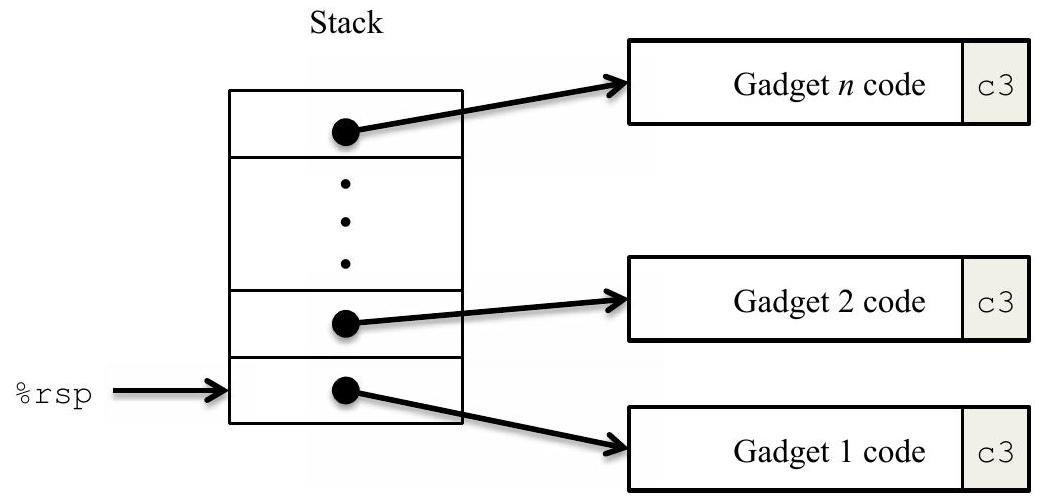
\includegraphics[max width=\textwidth]{attacklab_images/gadget.jpg}
\end{center}

그림 2: 실행을 위한 가젯 시퀀스 설정. 바이트 값 0xc3은 ret 명령을 인코딩합니다.
\noindent
이 그림에서 스택에는 일련의 가젯 주소가 포함되어 있습니다. 각 가젯은 일련의 인스트럭션 바이트로 구성되며, 마지막 바이트는 0xc3으로 ret 인스트럭션을 인코딩합니다. 프로그램이 이 구성으로 시작하는 ret 명령어를 실행하면 일련의 가젯 실행이 시작되며, 각 가젯의 끝에 있는 ret 명령어는 프로그램이 다음 가젯의 시작 부분으로 이동하도록 합니다.
\noindent
가젯은 컴파일러가 생성한 어셈블리 언어 문, 특히 함수 끝에 있는 문에 해당하는 코드를 사용할 수 있습니다. 실제로 이 형식의 유용한 가젯이 몇 가지 있을 수 있지만 많은 중요한 작업을 구현하기에는 충분하지 않습니다. 예를 들어, 컴파일된 함수의 마지막 인스트럭션이 ret 앞에 popq \%rdi가 있을 가능성은 거의 없습니다. 다행히도 x86-64와 같은 바이트 지향 명령어 집합에서는 명령어 바이트 시퀀스의 다른 부분에서 패턴을 추출하여 가젯을 찾을 수 있는 경우가 많습니다.
\noindent
예를 들어, 한 버전의 rtarget에는 다음 C 함수에 대해 생성된 코드가 포함되어 있습니다:


\begin{verbatim}
void setval_210(unsigned *p) 
{
    *p = 3347663060U;
}
\end{verbatim}
\noindent
이 함수가 시스템을 공격하는 데 유용할 가능성은 매우 희박해 보입니다. 하지만 이 함수의 머신 코드를 분해해 보면 흥미로운 바이트 시퀀스를 볼 수 있습니다:

\begin{verbatim}
0000000000400f15 <setval_210>:
    400f15: c7 07 d4 48 89 c7 movl $0xc78948d4,(%rdi)
    400f1b: c3 retq
\end{verbatim}
\noindent
바이트 시퀀스 4889c7은 movq 명령어 \%rax, \%rdi를 인코딩합니다. (유용한 movq 명령어의 인코딩은 그림 3A를 참조하세요.) 이 시퀀스 뒤에는 ret 명령어를 인코딩하는 바이트 값 c3이 이어집니다. 함수는 주소 0x400f15에서 시작하며, 시퀀스는 함수의 네 번째 바이트에서 시작됩니다. 따라서 이 코드에는 시작 주소가 0x400f15인 가젯이 포함되어 있으며, 이 가젯은 레지스터 \%rax의 64비트 값을 레지스터 \%rdi로 복사합니다.
\noindent
RTARGET에 대한 코드에는 가젯 팜이라고 하는 영역에 위에 표시된 setval 210 함수와 유사한 여러 함수가 포함되어 있습니다. 여러분의 임무는 가젯 팜에서 유용한 가젯을 식별하고 이를 사용하여 2단계와 3단계에서 수행한 것과 유사한 공격을 수행하는 것입니다.
\noindent
중요: 가젯 팜은 rtarget 사본에서 start\_farm 및 end\_farm 함수에 의해 구분됩니다. 프로그램 코드의 다른 부분에서 가젯을 구성하려고 시도하지 마세요.

\subsection*{5.1 Level 2}
4단계에서는 2단계의 공격을 반복하되, 가젯 팜의 가젯을 사용하여 RTARGET 프로그램에서 수행합니다. 다음 명령어 유형으로 구성된 가젯과 처음 8개의 x86=64 레지스터(\%rax-\%rdi)만 사용하여 솔루션을 구성할 수 있습니다.

movq : 이 명령어에 대한 코드는 그림 3A에 나와 있습니다.

popq : 이것들의 코드는 그림 3B에 나와 있습니다.

ret : 이 명령은 단일 바이트 0xc3으로 인코딩됩니다.

nop : 이 명령어("연산 없음"의 줄임말인 "no op"으로 발음)는 단일 바이트 0x90으로 인코딩됩니다. 이 명령의 유일한 효과는 프로그램 카운터를 1씩 증가시키는 것입니다.

\section*{조언:}
\begin{itemize}
  \item 필요한 모든 가젯은 start\_farm 및 mid\_farm 함수로 구분된 rtarget용 코드 영역에서 찾을 수 있습니다.
  \item 두 개의 가젯만으로 이 공격을 수행할 수 있습니다.
  \item 가젯이 popq 명령을 사용하면 스택에서 데이터를 pop합니다. 결과적으로 익스플로잇 문자열에는 가젯 주소와 데이터의 조합이 포함됩니다.
\end{itemize}

\subsection*{5.2 Level 3}
5단계를 시작하기 전에 잠시 멈춰서 지금까지 성취한 것을 생각해 보세요. 2단계와 3단계에서 여러분은 직접 설계한 머신 코드를 실행하는 프로그램을 만들었습니다. 만약 CTARGET이 네트워크 서버였다면, 여러분은 멀리 떨어진 컴퓨터에 직접 코드를 삽입할 수 있었을 것입니다. 4단계에서는 최신 시스템이 버퍼 오버플로 공격을 막기 위해 사용하는 두 가지 주요 장치를 우회했습니다. 직접 코드를 삽입하지는 않았지만, 기존 코드의 시퀀스를 연결하여 작동하는 일종의 프로그램을 삽입할 수 있었습니다. 또한 이 실습에서 95/100점을 받았습니다. 좋은 점수입니다. 다른 긴급한 의무가 있다면 지금 당장 중단하는 것이 좋습니다.
\noindent
5단계에서는 쿠키의 문자열 표현을 가리키는 포인터로 터치 3 함수를 호출하기 위해 RTARGET에 대한 ROP 공격을 수행해야 합니다. 이는 터치 2를 호출하기 위해 ROP 공격을 사용하는 것보다 크게 어렵지 않아 보일 수 있지만, 그렇게 만들었습니다. 게다가 5단계의 점수는 5점밖에 되지 않기 때문에 필요한 노력에 대한 진정한 척도가 아닙니다. 수업에 대한 일반적인 기대치를 뛰어넘고 싶은 분들을 위한 추가 점수 문제라고 생각하시면 됩니다.




















A. movq 명령어의 인코

\begin{center}
\begin{tabular}{|c|c|c|c|c|c|c|c|c|}
\hline
\begin{tabular}{c}
Source \\
S \\
\end{tabular} & \multicolumn{8}{|c|}{Destination D} \\
\hline
 & \%rax & \%rcx & \%rdx & \%rbx & \%rsp & \%rbp & \%rsi & \%rdi \\
\hline
\%rax & 48 89 c0 & 48 89 c1 & 48 89 c2 & 48 89 c3 & 48 89 c4 & 48 89 c5 & 48 89 c6 & 48 89 c7 \\
\hline
\%rcx & 48 89 c8 & 48 89 c9 & 48 89 ca & 48 89 cb & 48 89 cc & 48 89 cd & 48 89 ce & 48 89 cf \\
\hline
\%rdx & 48 89 d0 & 48 89 d1 & 48 89 d2 & 48 89 d3 & 48 89 d4 & 48 89 d5 & 48 89 d6 & 48 89 d7 \\
\hline
\%rbx & 48 89 d8 & 48 89 d9 & 48 89 da & 48 89 db & 48 89 dc & 48 89 dd & 48 89 de & 48 89 df \\
\hline
\%rsp & 48 89 e0 & 48 89 e1 & 48 89 e2 & 48 89 e3 & 48 89 e4 & 48 89 e5 & 48 89 e6 & 48 89 e7 \\
\hline
\%rbp & 48 89 e8 & 48 89 e9 & 48 89 ea & 48 89 eb & 48 89 ec & 48 89 ed & 48 89 ee & 48 89 ef \\
\hline
\%rsi & 48 89 f0 & 48 89 f1 & 48 89 f2 & 48 89 f3 & 48 89 f4 & 48 89 f5 & 48 89 f6 & 48 89 f7 \\
\hline
\%rdi & 48 89 f8 & 48 89 f9 & 48 89 fa & 48 89 fb & 48 89 fc & 48 89 fd & 48 89 fe & 48 89 ff \\
\hline
\end{tabular}
\end{center}

B. popq 명령어의 인코딩 

\begin{center}
\begin{tabular}{|c|c|c|c|c|c|c|c|c|}
\hline
Operation & \multicolumn{8}{|c|}{Register $R$} \\
\hline
 & \%rax & \%rcx & \%rdx & \%rbx & \%rsp & \%rbp & \%rsi & \%rdi \\
\hline
popq $R$ & 58 & 59 & 5a & 5b & 5c & 5d & 5e & 5f \\
\hline
\end{tabular}
\end{center}

C. movl 명령어의 인코딩 

movl S, D

\begin{center}
\begin{tabular}{|c|c|c|c|c|c|c|c|c|}
\hline
\begin{tabular}{c}
Source \\
$S$ \\
\end{tabular} & \multicolumn{8}{|c|}{Destination $D$} \\
\hline
 & \%eax & \%ecx & \%edx & \%ebx & \%esp & \%ebp & \%esi & \%edi \\
\hline
\%eax & 89 c0 & 89 c1 & 89 c2 & 89 c3 & 89 c4 & 89 c5 & 89 c6 & 89 c7 \\
\hline
\%ecx & 89 c8 & 89 c9 & 89 ca & 89 cb & 89 cc & 89 cd & 89 ce & 89 cf \\
\hline
\%edx & 89 d0 & 89 d1 & 89 d2 & 89 d3 & 89 d4 & 89 d5 & 89 d6 & 89 d7 \\
\hline
\%ebx & 89 d8 & 89 d9 & 89 da & 89 db & 89 dc & 89 dd & 89 de & 89 df \\
\hline
\%esp & 89 e0 & 89 e1 & 89 e2 & 89 e3 & 89 e4 & 89 e5 & 89 e6 & 89 e7 \\
\hline
\%ebp & 89 e8 & 89 e9 & 89 ea & 89 eb & 89 ec & 89 ed & 89 ee & 89 ef \\
\hline
\%esi & 89 f0 & 89 f1 & 89 f2 & 89 f3 & 89 f4 & 89 f5 & 89 f6 & 89 f7 \\
\hline
\%edi & 89 f8 & 89 f9 & 89 fa & 89 fb & 89 fc & 89 fd & 89 fe & 89 ff \\
\hline
\end{tabular}
\end{center}

D. 2바이트 nop 명령어의 인코딩 

\begin{center}
\begin{tabular}{|c|c|c|c|c|c|}
\hline
Operation & \multicolumn{4}{|c|}{Register $R$} \\
\hline
 &  & \%al & \%cl & \%dl & \%bl \\
\hline
andb & $R, \quad R$ & 20 c0 & 20 c9 & 20 d2 & 20 db \\
\hline
orb & $R, \quad R$ & 08 c0 & 08 c9 & 08 d2 & 08 db \\
\hline
cmpb & $R, \quad R$ & 38 c0 & 38 c9 & 38 d2 & 38 db \\
\hline
testb & $R, \quad R$ & 84 c0 & 84 c9 & 84 d2 & 84 db \\
\hline
\end{tabular}
\end{center}

Figure 3: 명령어의 바이트 인코딩. 모든 값은 16진수입니다. 
\noindent
5단계를 해결하려면 start\_farm 및 end\_farm 함수로 구분된 rtarget의 코드 영역에서 가젯을 사용할 수 있습니다. 4단계에서 사용된 가젯 외에도 이 확장된 팜에는 그림 3C에 표시된 것처럼 다양한 movl 명령어의 인코딩이 포함됩니다. 팜의 이 부분의 바이트 시퀀스에는 레지스터나 메모리 값을 변경하지 않는 기능적 NOP 역할을 하는 2바이트 명령어도 포함되어 있습니다. 여기에는 그림 3D에 표시된 것과 같이 일부 레지스터의 저차 바이트에서 작동하지만 해당 값을 변경하지 않는 명령어(예: andb \%al, \%al)가 포함됩니다.

\section*{Some Advice:}
\begin{itemize}
  \item CSAPP 책 183페이지에 설명된 대로 movl 명령어가 레지스터의 상위 4바이트에 미치는 영향을 검토하고 싶을 것입니다.
  \item 공식 솔루션에는 8개의 가젯이 필요합니다(모든 가젯이 고유하지는 않음).
\end{itemize}
\noindent
행운을 빌고 즐거운 시간 보내세요!

\section*{A - hex2raw 사용법}
HEX2RAW는 16진수 형식의 문자열을 입력으로 받습니다. 이 형식에서 각 바이트 값은 두 개의 16진수로 표시됩니다. 예를 들어, 문자열 "012345"는 "30 31 32 33 34 35 00"과 같이 16진수 형식으로 입력할 수 있습니다. (십진수 $x$의 ASCII 코드는 0x3$x$이며, 문자열의 끝은 널 바이트로 표시된다는 점을 기억하세요).
\noindent
HEX2RAW에 전달하는 16진수 문자는 공백(공백 또는 개행)으로 구분해야 합니다. 익스플로잇 문자열을 작업하는 동안 각 부분을 개행으로 구분하는 것이 좋습니다. HEX2RAW는 C-스타일 블록 주석을 지원하므로 익스플로잇 문자열의 섹션을 표시할 수 있습니다. 예를 들어

\begin{verbatim}
48 c7 c1 f0 11 40 00 /* mov $0x40011f0,%rcx */
\end{verbatim}
\noindent
주석이 제대로 무시될 수 있도록 시작과 끝 주석 문자열("/*", "*/") 주위에 공백을 남겨두어야 합니다.
\noindent
exploit.txt 파일에 16진수 형식의 익스플로잇 문자열을 생성한 경우, 여러 가지 방법으로 원시 문자열을 CTARGET 또는 RTARGET에 적용할 수 있습니다:

\begin{enumerate}
  \item 일련의 파이프를 설정하여 문자열이 HEX2RAW를 통과하도록 할 수 있습니다.
\end{enumerate}

\begin{verbatim}
    unix> cat exploit.txt | ./hex2raw | ./ctarget
\end{verbatim}

\begin{enumerate}
  \setcounter{enumi}{1}
  \item 원시 문자열을 파일에 저장하고 I/O 리디렉션을 사용할 수 있습니다:
\end{enumerate}

\begin{verbatim}
    unix> . /hex2raw < exploit.txt > exploit-raw.txt
    unix> ./ctarget < exploit-raw.txt
\end{verbatim}
\noindent
이 접근 방식은 GDB 내에서 실행할 때도 사용할 수 있습니다:

\begin{verbatim}
    unix > gdb ctarget
    (gdb) run < exploit-raw.txt
\end{verbatim}

\begin{enumerate}
  \setcounter{enumi}{2}
  \item 원시 문자열을 파일에 저장하고 파일 이름을 명령줄 인수로 제공할 수 있습니다:
\end{enumerate}

\begin{verbatim}
    unix> ./hex2raw < exploit.txt > exploit-raw.txt
    unix> ./ctarget -i exploit-raw.txt
\end{verbatim}
\noindent
이 접근 방식은 GDB 내에서 실행할 때도 사용할 수 있습니다.

\section*{B - 바이트코드 생성하는법}
어셈블러로 GCC를 사용하고 디스어셈블러로 OBJDUMP를 사용하면 명령어 시퀀스에 대한 바이트 코드를 편리하게 생성할 수 있습니다. 예를 들어 다음 어셈블리 코드가 포함된 example.s 파일을 작성한다고 가정해 보겠습니다:

\begin{verbatim}
# Example of hand-generated assembly code
    pushq $0xabcdef # Push value onto stack
    addq $17,%rax # Add 17 to %rax
    movl %eax,%edx # Copy lower 32 bits to %edx
\end{verbatim}
\noindent
코드에는 명령어와 데이터가 혼합되어 포함될 수 있습니다. '\#' 문자 오른쪽에 있는 것은 모두 주석입니다.
\noindent
이제 이 파일을 조립하고 분해할 수 있습니다:

\begin{verbatim}
    unix> gcc -c example.s
    unix> objdump -d example.o > example.d
\end{verbatim}
\noindent
생성된 파일 example.d에는 다음이 포함됩니다:

\begin{verbatim}
Disassembly of section .text:

0000000000000000 <.text>:
    0: 68 ef cd ab 00 pushq $0xabcdef
    5: 48 83 c0 11 add $0x11,%rax
    9: 89 c2 mov %eax,%edx
\end{verbatim}
\noindent
하단의 줄은 어셈블리 언어 명령어에서 생성된 머신 코드를 보여줍니다. 각 줄의 왼쪽에는 명령어의 시작 주소(0으로 시작)를 나타내는 16진수가 있으며, ':' 문자 뒤의 16진수는
': ' 문자 뒤의 16진수는 명령어의 바이트 코드를 나타냅니다. 따라서 명령 push \$0xABCDEF는 16진수 형식의 바이트 코드 68 ef cd ab 00임을 알 수 있습니다.
\noindent
이 파일에서 코드의 바이트 시퀀스를 얻을 수 있습니다:

\begin{verbatim}
68 ef cd ab 00 48 83 c0 11 89 c2
\end{verbatim}
\noindent
그런 다음 이 문자열을 HEX2RAW에 전달하여 대상 프로그램에 대한 입력 문자열을 생성할 수 있습니다. 또는 example.d를 편집하여 불필요한 값을 생략하고 가독성을 위해 C 스타일 주석을 포함하도록 하여 결과를 얻을 수 있습니다:

\begin{verbatim}
    68 ef cd ab 00 /* pushq $0xabcdef */
    48 83 c0 11 /* add $0x11,%rax */
    89 c2 /* mov %eax,%edx */
\end{verbatim}
\noindent
이는 대상 프로그램 중 하나로 보내기 전에 HEX2RAW를 통과할 수 있는 유효한 입력이기도 합니다.

\section*{참고문헌}
[1] R. Roemer, E. Buchanan, H. Shacham, and S. Savage. Return-oriented programming: Systems, languages, and applications. ACM Transactions on Information System Security, 15(1):2:1-2:34, March 2012.

\noindent
[2] E. J. Schwartz, T. Avgerinos, and D. Brumley. Q: Exploit hardening made easy. In USENIX Security Symposium, 2011.
\end{document}